\section{Analysis of the Evolution of a Single Atom}
  \label{sec:simultons_analysis}

    In order to understand the steep, early response in the \textsc{cw} probe
    signal observed in the experiment and matched in the numerical simulations, we
    turn in this section from the fields to focus on the evolution of the density
    matrix of a single atom as it is addressed by the probe and subsequently
    disturbed by the coupling pulse.

    As discussed in appendix \ref{apx:qu_dyn}, the density matrix $\rho$ is used
    to describe the state of an open quantum system such as an atom interacting
    both with coherent fields and with a stochastically modelled environment. We
    follow the evolution of $\rho$ using the Lindblad master equation
    (\ref{eqn:lindblad_apx}).

    The Hamiltonian for the V-type atom was given in equation
    (\ref{eqn:vee_hamiltonian}). In the case of the pulsed coupling scheme, at the
    front of the medium we have input time-dependent fields $\Omega_p(t)$ and
    $\Omega_c(t)$ and thus a time-dependent Hamiltonian
    $\mathcal{H}_\mathrm{V}(t)$. We can solve the the Lindblad equation
    numerically given an initial condition.

    We imagine the \textsc{cw} probe having plenty of time to equilibrate before
    the pulse, so we first find the steady state solution with the probe on and
    the coupling pulse off. This steady state constitutes the initial condition.

    \begin{figure}
    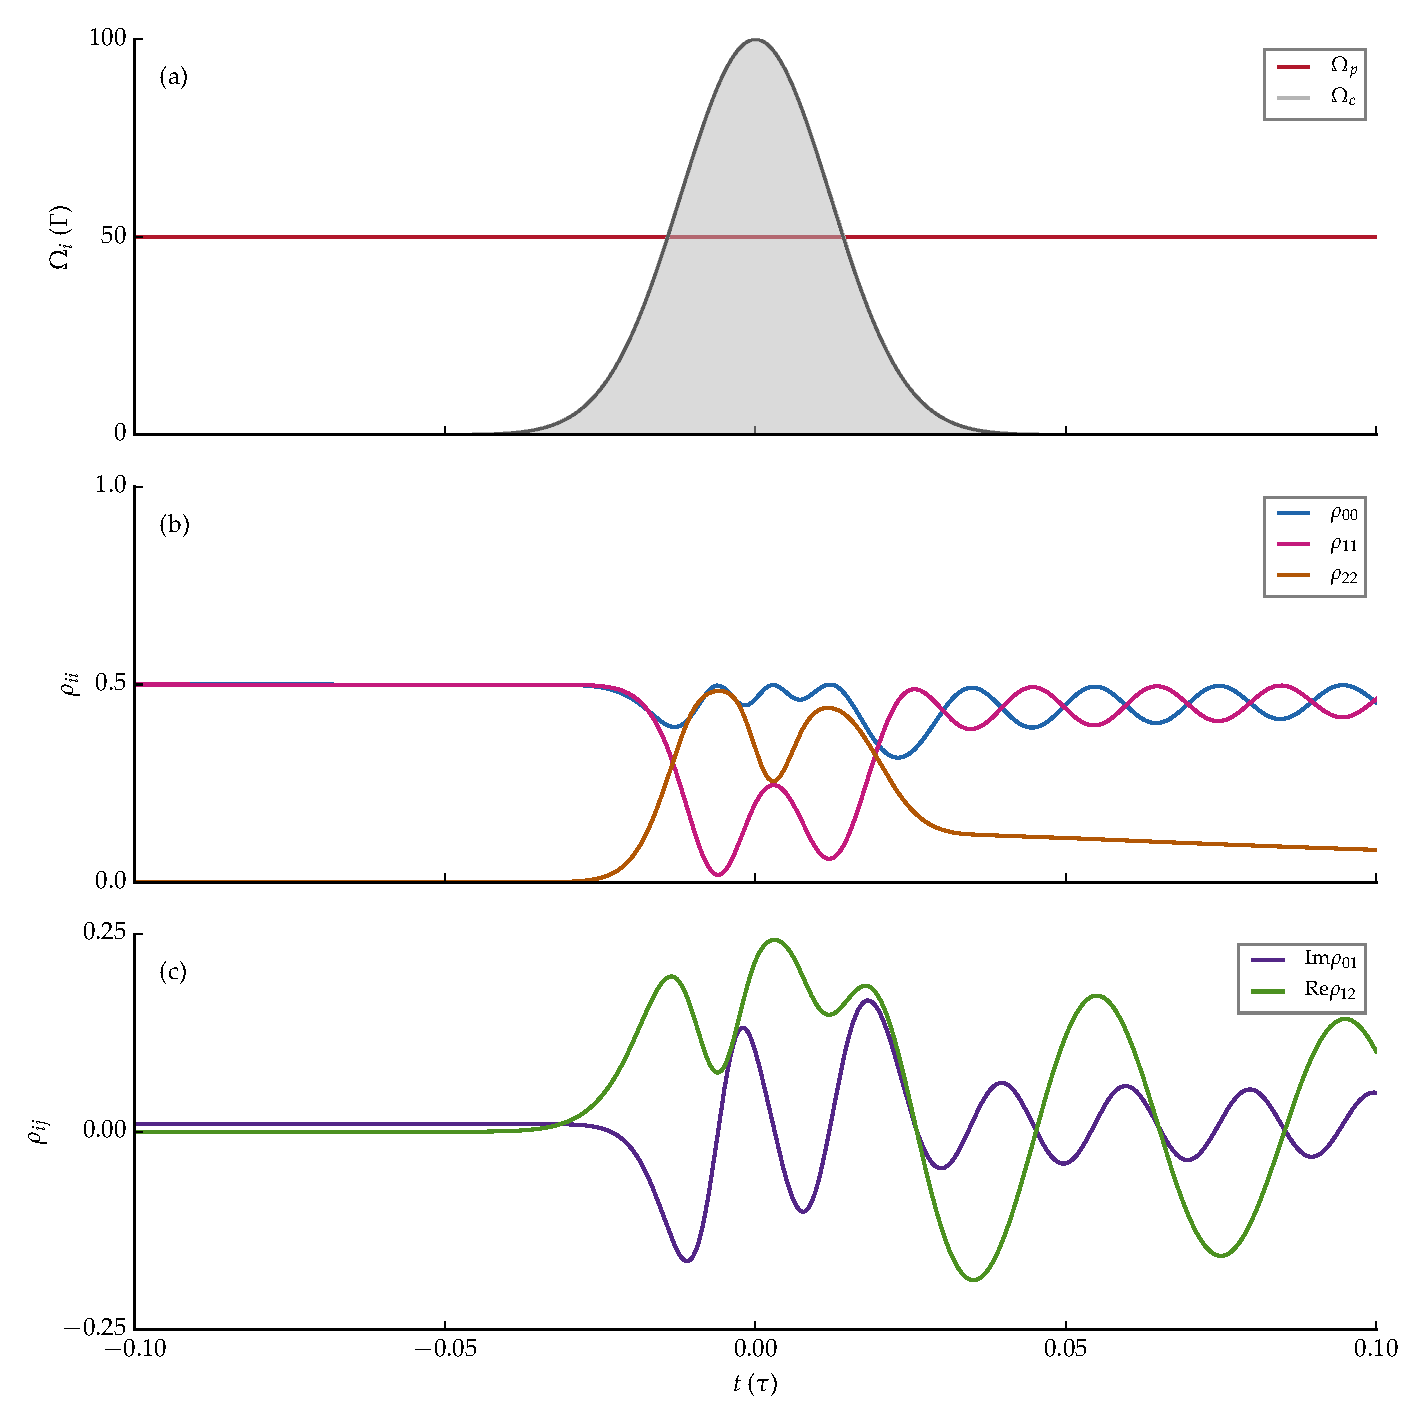
\includegraphics[width=\linewidth]{figs/06_simultons/ob_vee_solve_pls_t002_50c_100p_fig1.pdf}
    \caption{
    Time evolution of the density matrix elements from numerical solution of the
    master equation for the V configuration atom.  (a) Rabi frequency profiles
    of the two fields: a \textsc{cw} probe $\Omega_p$ (red) and Gaussian pulsed
    coupling $\Omega_c$ (grey) with amplitude $\unit[2\pi\times100]\Gamma$ and width $t_w
    = $ \unit[0.02]{$\tau_\Gamma$}. (b) Populations of the atomic eigenstates.
    (c) The imaginary part of coherence $\rho_{01}$ (purple) and the real part
    of coherence $\rho_{12}$ (green).
    }
    \label{fig:ob_vee_pulse}
    \end{figure}

    In figure \ref{fig:ob_vee_pulse} we show the time evolution of density
    matrix populations and coherences for an example Gaussian pulse profile of
    peak $\unit[100]\Gamma$ and width \unit[0.02]{$\tau_\Gamma$}, where here
    we ll assume $\Gamma := \Gamma_{01} = \Gamma_{02}$ and define $\tau_\Gamma
    := \nicefrac{1}{\Gamma}$ as the reciprocal lifetime. The \textsc{cw} probe
    Rabi frequency is $\unit[50]\Gamma$. Before the pulse, the steady state
    population is an even split between $\rho_{00}$ and $\rho_{11}$. As the
    pulse ramps on we see it coherently drive population transfer such that it
    oscillates between populations $\rho_{11}$ and $\rho_{22}$. This is
    accompanied by a positive real coherence $\rho_{12}$, and an imaginary
    coherence $\rho_{01}$ which oscillates first negative and then positive.
    After the pulse we see damped oscillation of $\rho_{00}$ and $\rho_{11}$,
    and at long times we expect the system to return to its steady state.

    The behaviour of the imaginary part of $\rho_{01}$ is of particular interest
    as we know that the macroscopic consequence of this atomic coherence is
    polarisation of the medium with respect to the probe field, and resulting
    attenuation or amplification of that field. From the observed evolution we
    can then predict that during the pulse, without the populations $\Ket{0}$
    and $\Ket{1}$ being inverted, we will find reduced absorption and possibly
    gain in the probe field.

    To understand this time evolution, we write out the components of equation
    (\ref{eqn:lindblad}) for the V configuration to get a set of differential
    equations for the density matrix elements
    \begin{subequations}
    \begin{align}
    \frac{\partial \rho_{00}}{\partial t} &= \Gamma_{01} \rho_{11} + \Gamma_{02} 
    \rho_{22} + \frac{\ii}{2} \bigg[ \Omega_p 
    ( \rho_{01} - \rho_{10}) + \Omega_c ( \rho_{02} - \rho_{20}) \bigg] \\
    \frac{\partial \rho_{01}}{\partial t} &= -\frac{\Gamma_{01}}{2} \rho_{01} - 
    \ii \Delta_1 \rho_{01} + \frac{\ii}{2} \bigg[ \Omega_p 
    (\rho_{00} - \rho_{11}) - \Omega_c \rho_{21} \bigg] \\
    \frac{\partial \rho_{02}}{\partial t} &= -\frac{\Gamma_{02}}{2} \rho_{02} - 
    \ii \Delta_2 \rho_{02} + \frac{\ii}{2} \bigg[ -\Omega_p \rho_{12} + \Omega_c 
    ( \rho_{00} - \rho_{22} ) \bigg] \\
    \frac{\partial \rho_{11}}{\partial t} &= -\Gamma_{01} \rho_{11} - 
    \frac{\ii}{2} \Omega_p (\rho_{01} - \rho_{10}) \\
    \frac{\partial \rho_{12}}{\partial t} &= -\frac{\Gamma_{01}}{2} \rho_{12} - 
    \frac{\Gamma_{02}}{2} \rho_{12} + \ii (\Delta_1 - \Delta_2) \rho_{12} - 
    \frac{\ii}{2} (\Omega_p \rho_{02} - \Omega_c{\rho_{10}})\\
    \frac{\partial \rho_{22}}{\partial t} &= -\frac{\Gamma_{02}}{2} \rho_{22} - 
    \frac{\ii}{2} \Omega_c ( \rho_{02} - \rho_{20} ).
    \end{align}
    \label{eqn:vee_dm_equations}
    \end{subequations}
    Note that $\rho_{10} = \rho_{01}^\dagger$ and $\rho_{20} =
    \rho_{02}^\dagger$.

    Starting with equation (\ref{eqn:vee_dm_equations}e) we see that in the case
    of two-photon resonance ($\Delta_1 = \Delta_2 = 0$) and in the steady state
    at the start of the pulse
    \begin{equation}
       \frac{\partial \rho_{12}(t_{0})}{\partial t} \approx \frac{\ii}{2} 
        \Omega_c(t_{0}) \rho_{10}(t_{0}).
      \label{eqn:rho12}
    \end{equation}
    The steady state $\rho_{10}$ for the two-level system is
    positive imaginary, thus $\rho_{12}$ is initially driven real and positive
    by the pulse.

    If we next look at equation (\ref{eqn:vee_dm_equations}b), we see that again
    on resonance and in the steady state with $\rho_{11} = \rho_{00}$
    \begin{equation}
       \frac{\partial \rho_{01}(t_{0})}{\partial t} \approx -\frac{\ii}{2} 
        \Omega_c \rho_{21}
      \label{eqn:rho01}
    \end{equation}
    such that with $\rho_{21}$ real and positive $\rho_{01}$ is driven imaginary
    and negative. This is consistent with the behaviour observed in the
    evolution of coherences in figure \ref{fig:ob_vee_pulse}.

  \subsection{Coherent Population Trapping}

    We may gain further insight into the transient effect of the pulse on the
    system by considering the eigenstates of the atom dressed by the fields,
    that is the eigenvectors of $\mathcal{H}_\mathrm{V}$.\cite{lambropoulos2007fundamentals, Blok1990} If we consider equal
    detunings $\Delta := \Delta_p = \Delta_c$ and solve for
    $\mathcal{H}_\mathrm{V} \Ket{\psi} = \hbar \lambda \Ket{\psi}$ we find
    eigenvalues
    \begin{subequations}
      \begin{align}
      \lambda_0 &= -\Delta \\
      \lambda_\pm &= \frac{-\Delta \pm \bar{\Omega}}{2}
      \end{align}
      \label{eqn:vee_eigvals}
    \end{subequations}
    where $\bar{\Omega}= \sqrt{\Omega_p^2 + \Omega_c^2 + \Delta^2}$. These
    eigenvalues have corresponding normalised eigenstates
    \begin{subequations}
      \begin{align}
      \Ket{D} &= \frac{1}{\sqrt{N_0}} \big( -\Omega_c \Ket{1} + \Omega_p 
      \Ket{2} \big) \\
      \Ket{B_\pm} &= \frac{1}{\sqrt{N_\pm}} \big(-2 \lambda_\mp \Ket{0} + 
      \Omega_p \Ket{1} + \Omega_c \Ket{2} \big)
      \end{align}
      \label{eqn:vee_eigvects}
    \end{subequations}
    where $N_0 := \Omega_p^2 + \Omega_c^2$ and $N_\pm := N_0 + 4 \lambda_\mp^2$.

    Note that the energy eigenvalue $\lambda_0$ is zero on resonance. For this
    reason, its corresponding eigenstate $\Ket{D}$, which does not contain any
    component of the ground state and so is decoupled from the fields, is known
    as a dark state. Any population entering the dark state cannot be driven out
    again by the coherent fields, it can only decay spontaneously. This
    phenomenon is known as coherent population trapping
    (\textsc{cpt}).\cite{Fleischhauer2005} The states $\Ket{B_\pm}$, which are
    coupled to the fields, are known as bright states.

    We can transform from the bare state density matrix $\rho$ to the similar
    \textsc{cpt} state density matrix $\rho'$ via
    \begin{equation}
      \rho' = \mathcal{T}^{-1} \rho \mathcal{T}
      \label{eqn:rho01}
    \end{equation}
    where $\mathcal{T}$ is the unitary transform defined by equations
    (\ref{eqn:vee_eigvects}).

    \begin{figure}[]
    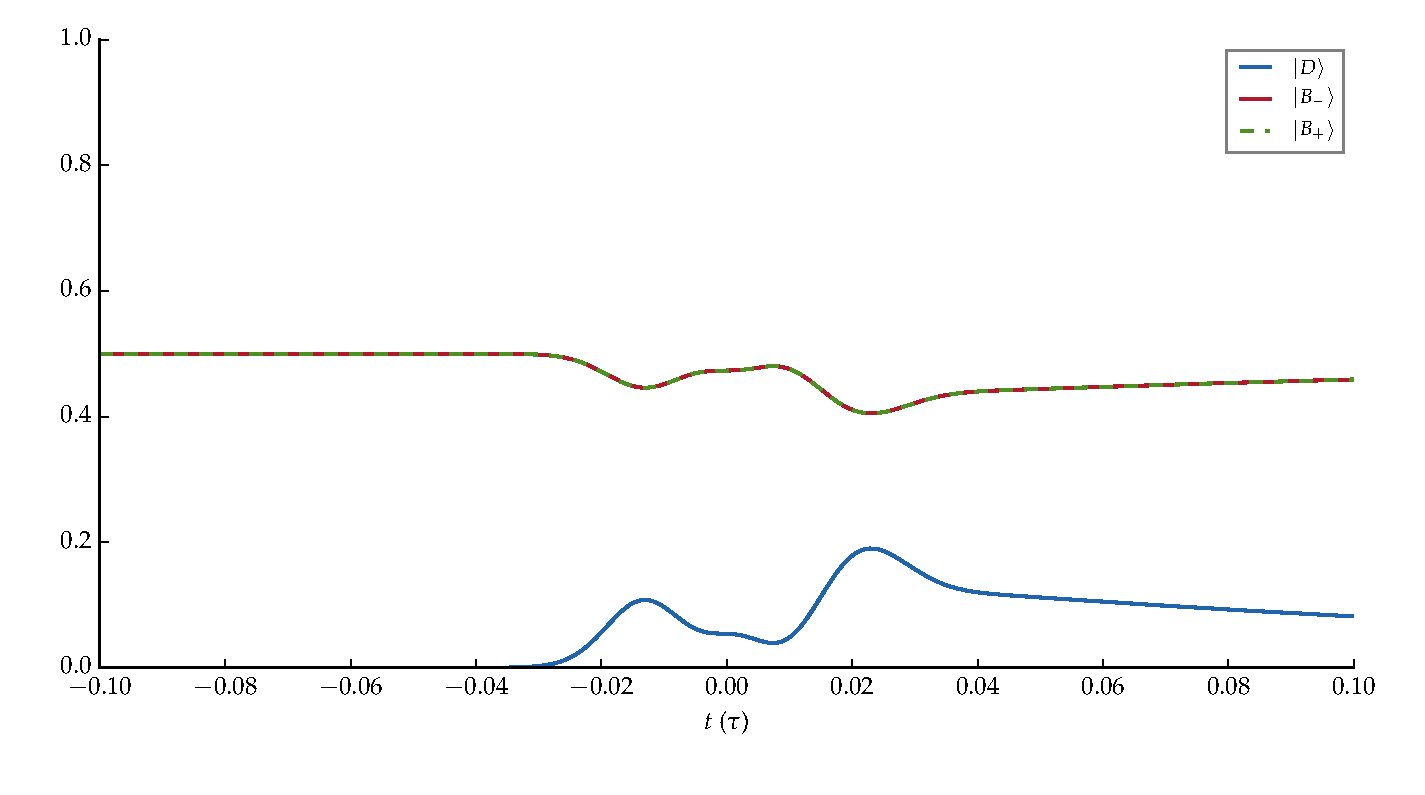
\includegraphics[width=\linewidth]{figs/06_simultons/ob_vee_solve_pls_t002_50c_100p_fig2.pdf}
    \caption{
    Time evolution of the populations of the \textsc{cpt} state populations
    $\Ket{D}$ (blue), $\Ket{B_-}$ (red) and $\Ket{B_+}$ (green dashed) for the
    V-type atom addressed by a coupling pulse with amplitude $\unit[100]\Gamma$
    and width $t_w = $ \unit[0.02]{$\tau_\Gamma$}.
    }
    \label{fig:wp_propagation} 
    \end{figure}

    In figure \ref{fig:wp_propagation}, we show the time evolution of the
    populations of the \textsc{cpt} states $\Ket{D}$ and $\Ket{B_\pm}$ during
    the pulse shown in figure \ref{fig:ob_vee_pulse} for the bare states. We see
    that during the pulse, an amount of population is driven into the dark state
    $\Ket{D}$, where it will be trapped. As the population is trapped the
    absorption in the medium is reduced, thus allowing part of the field to
    propagate further into the medium than it would otherwise.

    In summary, in this section we have analysed the time evolution of the
    atomic states in both the bare and \textsc{cpt} basis during the pulse. We
    found that the strong pulse drives an oscillation, first negative, in the
    imaginary part of $\rho_{01}$, which we expect to cause a reduction in
    absorption of the probe beam due to the relation of this coherence to the
    macroscopic polarisation of the medium.

    These findings are consistent with the observed signal increase in the probe
    beam during the early part of the pulse. It does not, however, explain the
    increase in the signal response with increased temperature. For a complete
    understanding of the behaviour, we will next move on to considering the
    effects of pulse propagation and investigate what would happen if we extend
    the simulations to longer propagation distances.

    


